
%!TEX program = xelatex
\documentclass{ctexart}
\usepackage{graphicx}
\usepackage{amsmath}

\title{实验二:粒子群优化算法实验}
\author{罗耀辉}
\date{2024-05-8}

\begin{document}

\maketitle

\section{实验内容}
粒子群优化算法编写。

\section{实验要求}
\begin{enumerate}
    \item 选择连续或离散的粒子群优化算法编写代码,并解决一个优化问题;
    \item 提交实验报告,报告内容包括算法思想、算法流程,以及解决问题的结果分析。
\end{enumerate}

\section{求解的问题}
本实验旨在使用粒子群优化算法(PSO)求解一个简单的函数优化问题。具体来说,我们希望找到函数 $f(x, y) = x^2 + y^2$ 的最小值。这个函数在 $(0, 0)$ 处取得全局最小值,最小值为 $0$。

\section{算法原理}
粒子群优化算法(Particle Swarm Optimization, PSO)是一种基于群体智能的优化算法,起源于对鸟群觅食行为的模拟。PSO通过模拟粒子在搜索空间中的移动,利用个体经验和群体经验找到全局最优解。每个粒子都有一个位置和速度,通过不断更新位置和速度来搜索最优解。

\section{算法思想}
PSO算法的基本思想是通过模拟粒子在搜索空间中的飞行,利用个体和群体的最佳位置来指导粒子的搜索方向。每个粒子的位置和速度更新公式如下:

\begin{equation}
v_{i}(t+1) = w \cdot v_{i}(t) + c_{1} \cdot r_{1} \cdot (p_{i}(t) - x_{i}(t)) + c_{2} \cdot r_{2} \cdot (g(t) - x_{i}(t))
\end{equation}

\begin{equation}
x_{i}(t+1) = x_{i}(t) + v_{i}(t+1)
\end{equation}

其中,$v_{i}(t)$ 和 $x_{i}(t)$ 分别表示粒子 $i$ 在时间 $t$ 的速度和位置;$w$ 是惯性权重,表示粒子保持其运动方向的能力;$c_{1}$ 和 $c_{2}$ 是加速常数,分别表示个体和群体的学习因子;$r_{1}$ 和 $r_{2}$ 是在 [0,1] 之间的随机数;$p_{i}(t)$ 是粒子 $i$ 的历史最优位置;$g(t)$ 是全体粒子的全局最优位置。

\section{算法流程}
\begin{enumerate}
    \item 初始化粒子的位置和速度;
    \item 计算每个粒子的适应度;
    \item 更新每个粒子的速度和位置;
    \item 更新全局最优解;
    \item 判断是否满足终止条件,若满足则输出最优解,否则继续迭代。
\end{enumerate}

\section{算法参数}
\begin{itemize}
    \item 惯性权重($w$):控制粒子速度的惯性,值为 0.5。
    \item 个体学习因子($c_1$):引导粒子向自身最佳位置移动的加速常数,值为 1.5。
    \item 群体学习因子($c_2$):引导粒子向群体最佳位置移动的加速常数,值为 1.5。
    \item 粒子数量:30 个。
    \item 维度(dim):2 维,即 $x$ 和 $y$。
    \item 迭代次数:200 次。
\end{itemize}

\section{代码实现}
以下是粒子群优化算法的Python实现代码:

\begin{verbatim}
# -*- coding: utf-8 -*-
import numpy as np
import matplotlib.pyplot as plt
from mpl_toolkits.mplot3d import Axes3D

# 定义粒子类
class Particle:
    def __init__(self, dim):
        self.position = np.random.rand(dim) * 20 - 10  # 初始化位置在[-10, 10]范围内
        self.velocity = np.random.rand(dim) - 0.5  # 初始化速度
        self.best_position = self.position.copy()  # 初始化个体最佳位置
        self.best_value = float('inf')  # 初始化个体最佳值

# 适应度函数,求解目标函数值
def fitness_function(x):
    return np.sum(x**2)  # 简单的平方和函数

# 粒子群优化算法
def pso(num_particles, dim, num_iterations):
    particles = [Particle(dim) for _ in range(num_particles)]  # 初始化粒子群
    global_best_position = np.random.rand(dim) * 20 - 10  # 初始化全局最佳位置
    global_best_value = float('inf')  # 初始化全局最佳值
    fitness_values = []  # 用于存储每次迭代的全局最优值

    for _ in range(num_iterations):
        for particle in particles:
            value = fitness_function(particle.position)  # 计算适应度值
            if value < particle.best_value:  # 更新个体最佳值和位置
                particle.best_value = value
                particle.best_position = particle.position.copy()
            if value < global_best_value:  # 更新全局最佳值和位置
                global_best_value = value
                global_best_position = particle.position.copy()
            
            # 更新速度和位置
            w = 0.5  # 惯性权重
            c1 = c2 = 1.5  # 学习因子
            r1 = r2 = np.random.rand(dim)  # 随机数
            cognitive = c1 * r1 * (particle.best_position - particle.position)
            social = c2 * r2 * (global_best_position - particle.position)
            particle.velocity = w * particle.velocity + cognitive + social
            particle.position += particle.velocity
        
        fitness_values.append(global_best_value)  # 记录全局最优值
    
    return global_best_position, global_best_value, fitness_values

# 运行粒子群优化算法
best_position, best_value, fitness_values = pso(num_particles=30, dim=2, num_iterations=200)
print(f"最佳位置: {best_position}")
print(f"最佳值: {best_value}")

# 绘制适应度变化曲线
plt.figure(figsize=(14, 6))

plt.subplot(1, 2, 1)
plt.plot(fitness_values)
plt.title('适应度变化曲线')
plt.xlabel('迭代次数')
plt.ylabel('适应度值')

# 绘制三维函数图
x = np.linspace(-10, 10, 400)
y = np.linspace(-10, 10, 400)
X, Y = np.meshgrid(x, y)
Z = X**2 + Y**2

ax = plt.subplot(1, 2, 2, projection='3d')
ax.plot_surface(X, Y, Z, cmap='viridis', alpha=0.7)
ax.scatter(best_position[0], best_position[1], best_value, color='r', marker='o', s=100)
ax.set_title('三维适应度函数图')
ax.set_xlabel('X')
ax.set_ylabel('Y')
ax.set_zlabel('适应度值')

# 保存图像
plt.savefig('pso_results.png')

# 显示图像
plt.show()
\end{verbatim}

\section{结果分析}
通过运行上述粒子群优化算法,我们得到了最佳位置和最佳值。具体结果如下:

\begin{itemize}
    \item 最佳位置:\texttt{[8.27718794e-18, 5.09844422e-19]}
    \item 最佳值:\texttt{6.877178148439595e-35}
\end{itemize}

\begin{figure}[h!]
    \centering
    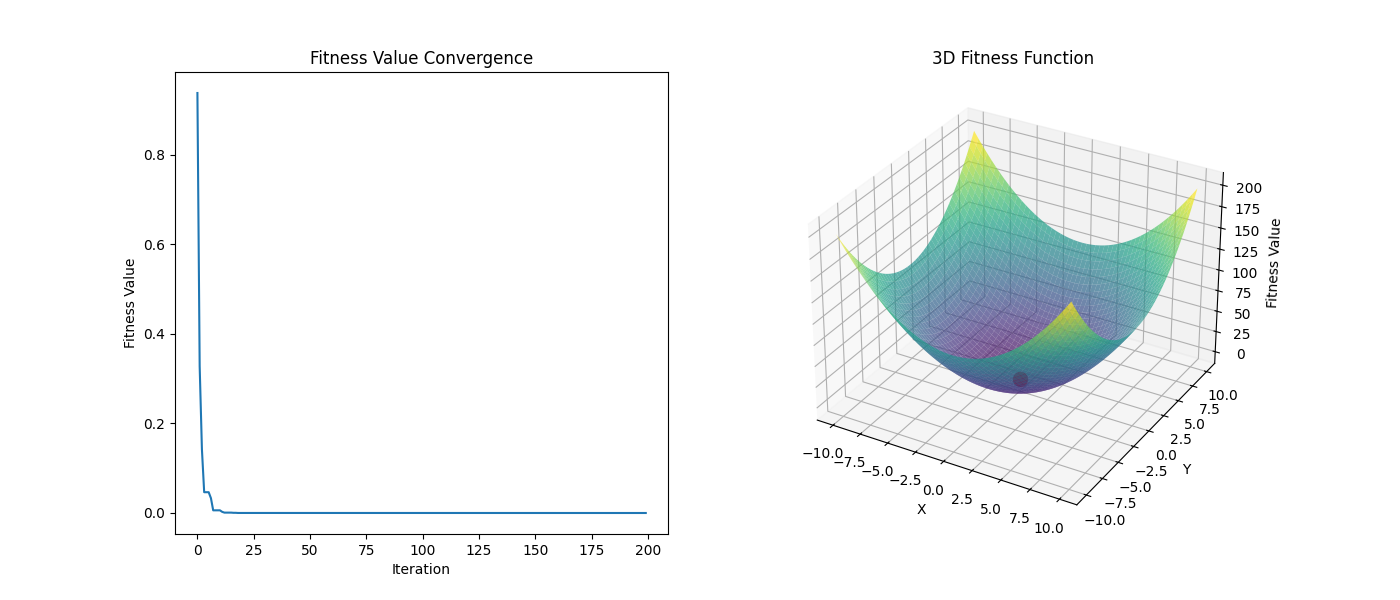
\includegraphics[width=0.8\textwidth]{pso_results.png}
    \caption{适应度变化曲线和三维适应度函数图}
    \label{fig:pso_results}
\end{figure}

\section{结论}
粒子群优化算法是一种简单且有效的优化方法,适用于多种优化问题。通过调整算法参数,可以在不同问题中取得良好效果。该实验展示了粒子群优化算法在求解简单函数优化问题上的有效性。

\end{document}
